\chapter{Energy Ratios: $E_s/N_0$ and $E_b/N_0$}
\label{ch:energy-ratios}

\begin{nontechnical}
\textbf{$E_s/N_0$ and $E_b/N_0$ are like measuring ``signal strength per bit'' compared to background noise}---higher ratio = cleaner signal = fewer errors!

\textbf{Think of it like listening to a radio:}
\begin{itemize}
\item \textbf{Energy} ($E_b$ or $E_s$) = How loud/strong each bit or symbol is
\item \textbf{Noise} ($N_0$) = Static and interference level
\item \textbf{Ratio} = Signal clarity measure
\end{itemize}

\textbf{Two related measurements:}
\begin{itemize}
\item \textbf{$E_b/N_0$} (energy per BIT): Used to fairly compare different systems
\item \textbf{$E_s/N_0$} (energy per SYMBOL): Used for actual performance calculations
\end{itemize}

\textbf{Real-world WiFi example:}
\begin{itemize}
\item Close to router: $E_b/N_0 = 25$~dB $\rightarrow$ use 256-QAM (fast!)
\item Far from router: $E_b/N_0 = 10$~dB $\rightarrow$ use QPSK (reliable!)
\item Too far: $E_b/N_0 = 5$~dB $\rightarrow$ connection drops
\end{itemize}

\textbf{Fun fact:} The theoretical minimum $E_b/N_0$ for error-free communication is $-1.59$~dB (Shannon limit), but real systems need 5--15~dB due to practical limitations!
\end{nontechnical}

\section{Overview}

Energy ratios are the fundamental metrics for characterizing communication system performance in the presence of noise. Unlike simple signal-to-noise ratio (SNR), which measures power ratios, energy ratios normalize by the information rate, enabling fair comparison between different modulation schemes and coding strategies.

\begin{keyconcept}
\textbf{$E_b/N_0$} is the universal metric for comparing communication systems. It represents the energy per information bit relative to the noise spectral density, independent of data rate, bandwidth, or modulation scheme. All theoretical capacity limits and practical system specifications are referenced to $E_b/N_0$.
\end{keyconcept}

\section{Mathematical Description}

\subsection{Energy per Bit: $E_b$}

The energy per bit is the total signal energy transmitted per information bit:
\begin{equation}
E_b = P_s \cdot T_b
\end{equation}
where:
\begin{itemize}
\item $E_b$ = energy per bit (joules)
\item $P_s$ = average signal power (watts)
\item $T_b$ = bit duration (seconds)
\end{itemize}

Equivalently, in terms of bit rate $R_b$:
\begin{equation}
E_b = \frac{P_s}{R_b}
\end{equation}
where $R_b = 1/T_b$ is the bit rate in bits per second.

\subsection{Energy per Symbol: $E_s$}

For modulation schemes transmitting $k$ bits per symbol:
\begin{equation}
E_s = P_s \cdot T_s = P_s \cdot k T_b
\end{equation}
where:
\begin{itemize}
\item $E_s$ = energy per symbol (joules)
\item $T_s$ = symbol duration (seconds)
\item $k$ = bits per symbol
\end{itemize}

\subsection{Noise Spectral Density: $N_0$}

The noise spectral density represents noise power per unit bandwidth:
\begin{equation}
N_0 = \frac{P_n}{B}
\end{equation}
where:
\begin{itemize}
\item $N_0$ = noise power spectral density (W/Hz)
\item $P_n$ = total noise power (watts)
\item $B$ = noise bandwidth (Hz)
\end{itemize}

For thermal noise (additive white Gaussian noise):
\begin{equation}
N_0 = k_B T
\end{equation}
where:
\begin{itemize}
\item $k_B = 1.38 \times 10^{-23}$~J/K (Boltzmann's constant)
\item $T$ = system noise temperature (kelvin)
\end{itemize}

\begin{calloutbox}{Example: Room Temperature Noise}
At room temperature ($T = 290$~K):
\begin{equation}
N_0 = (1.38 \times 10^{-23})(290) = 4.0 \times 10^{-21}~\text{W/Hz} = -174~\text{dBm/Hz}
\end{equation}
This is the fundamental noise floor for all room-temperature receivers.
\end{calloutbox}

\subsection{The $E_b/N_0$ Ratio}

The energy per bit to noise spectral density ratio is:
\begin{equation}
\frac{E_b}{N_0} = \frac{P_s \cdot T_b}{N_0} = \frac{P_s}{N_0 \cdot R_b}
\end{equation}

In decibels:
\begin{equation}
\frac{E_b}{N_0}\bigg|_{\text{dB}} = 10\log_{10}\left(\frac{E_b}{N_0}\right)
\end{equation}

\subsection{The $E_s/N_0$ Ratio}

Similarly, for symbol energy:
\begin{equation}
\frac{E_s}{N_0} = \frac{P_s \cdot T_s}{N_0} = \frac{P_s}{N_0 \cdot R_s}
\end{equation}
where $R_s = 1/T_s$ is the symbol rate.

\subsection{Relationship Between $E_s/N_0$ and $E_b/N_0$}

Since $E_s = k \cdot E_b$ (where $k$ = bits per symbol):
\begin{equation}
\frac{E_s}{N_0} = k \cdot \frac{E_b}{N_0}
\end{equation}

In decibels:
\begin{equation}
\frac{E_s}{N_0}\bigg|_{\text{dB}} = \frac{E_b}{N_0}\bigg|_{\text{dB}} + 10\log_{10}(k)
\end{equation}

Or equivalently:
\begin{equation}
\frac{E_b}{N_0}\bigg|_{\text{dB}} = \frac{E_s}{N_0}\bigg|_{\text{dB}} - 10\log_{10}(k)
\end{equation}

\textbf{Common conversions:}
\begin{center}
\begin{tabular}{@{}lll@{}}
\toprule
Modulation & $k$ (bits/symbol) & Conversion (dB) \\
\midrule
BPSK & 1 & $E_b/N_0 = E_s/N_0 - 0.00$ \\
QPSK & 2 & $E_b/N_0 = E_s/N_0 - 3.01$ \\
8PSK & 3 & $E_b/N_0 = E_s/N_0 - 4.77$ \\
16-QAM & 4 & $E_b/N_0 = E_s/N_0 - 6.02$ \\
64-QAM & 6 & $E_b/N_0 = E_s/N_0 - 7.78$ \\
\bottomrule
\end{tabular}
\end{center}

\section{Visualization}

\subsection{Energy per Bit and Symbol}

The relationship between bit energy, symbol energy, and modulation order is visualized below:

\begin{center}
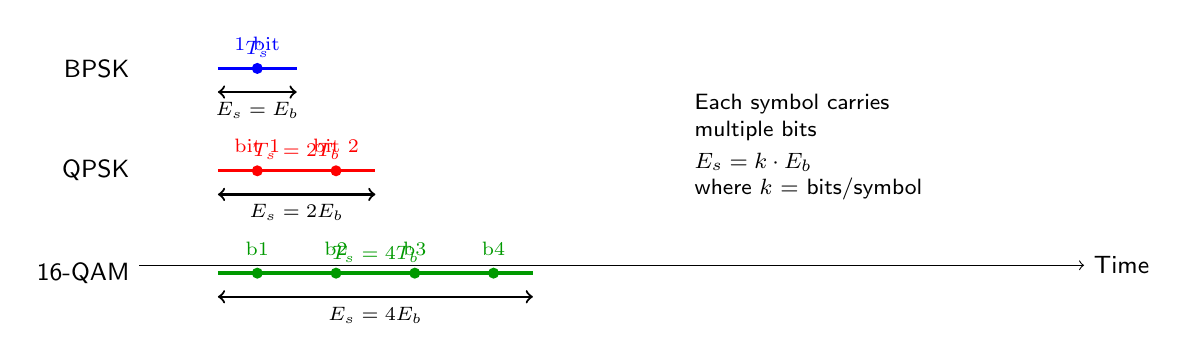
\begin{tikzpicture}[scale=1.0]
% Time axis
\draw[->] (0,0) -- (12,0) node[right,font=\sffamily\small] {Time};

% BPSK example (1 bit per symbol)
\node[left,font=\sffamily\small] at (0,2.5) {BPSK};
\draw[very thick,blue] (1,2.5) -- (2,2.5) node[midway,above,font=\scriptsize] {$T_s$};
\draw[<->,thick] (1,2.2) -- (2,2.2) node[midway,below,font=\scriptsize] {$E_s = E_b$};
\fill[blue] (1.5,2.5) circle (2pt) node[above,font=\scriptsize,yshift=3pt] {1 bit};

% QPSK example (2 bits per symbol)
\node[left,font=\sffamily\small] at (0,1.2) {QPSK};
\draw[very thick,red] (1,1.2) -- (3,1.2) node[midway,above,font=\scriptsize] {$T_s = 2T_b$};
\draw[<->,thick] (1,0.9) -- (3,0.9) node[midway,below,font=\scriptsize] {$E_s = 2E_b$};
\fill[red] (1.5,1.2) circle (2pt) node[above,font=\scriptsize,yshift=3pt] {bit 1};
\fill[red] (2.5,1.2) circle (2pt) node[above,font=\scriptsize,yshift=3pt] {bit 2};

% 16-QAM example (4 bits per symbol)
\node[left,font=\sffamily\small] at (0,-0.1) {16-QAM};
\draw[very thick,green!60!black] (1,-0.1) -- (5,-0.1) node[midway,above,font=\scriptsize] {$T_s = 4T_b$};
\draw[<->,thick] (1,-0.4) -- (5,-0.4) node[midway,below,font=\scriptsize] {$E_s = 4E_b$};
\fill[green!60!black] (1.5,-0.1) circle (2pt) node[above,font=\scriptsize,yshift=3pt] {b1};
\fill[green!60!black] (2.5,-0.1) circle (2pt) node[above,font=\scriptsize,yshift=3pt] {b2};
\fill[green!60!black] (3.5,-0.1) circle (2pt) node[above,font=\scriptsize,yshift=3pt] {b3};
\fill[green!60!black] (4.5,-0.1) circle (2pt) node[above,font=\scriptsize,yshift=3pt] {b4};

% Legend
\node[font=\sffamily\footnotesize,align=left] at (8.5,1.5) {
  Each symbol carries\\
  multiple bits\\[2pt]
  $E_s = k \cdot E_b$\\
  where $k$ = bits/symbol
};

\end{tikzpicture}
\end{center}

\subsection{Noise Spectral Density}

The noise spectral density $N_0$ represents the noise power distributed across frequency:

\begin{center}
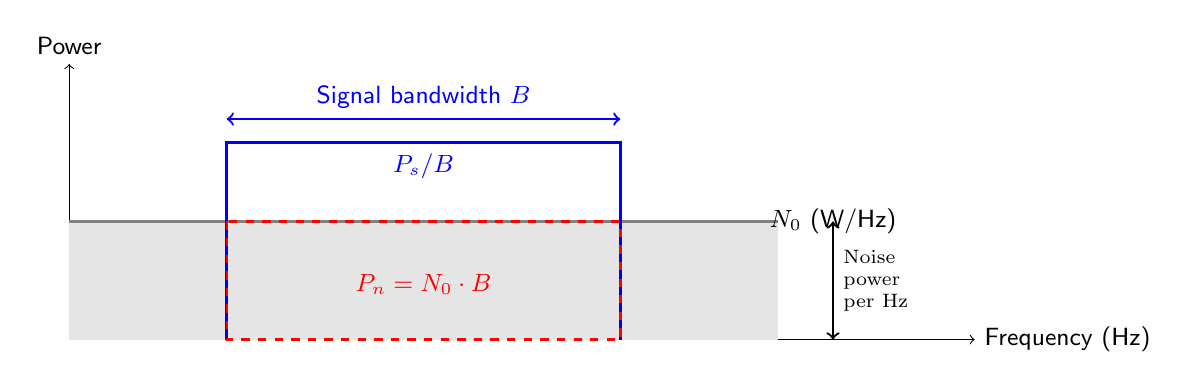
\begin{tikzpicture}[scale=1.0]
% Frequency axis
\draw[->] (0,0) -- (11.5,0) node[right,font=\sffamily\small] {Frequency (Hz)};
\draw[->] (0,0) -- (0,3.5) node[above,font=\sffamily\small] {Power};

% Noise floor
\fill[gray!20] (0,0) rectangle (9,1.5);
\draw[thick,gray] (0,1.5) -- (9,1.5);
\node[font=\sffamily\small] at (9.7,1.5) {$N_0$ (W/Hz)};

% Signal bandwidth
\draw[<->,thick,blue] (2,2.8) -- (7,2.8) node[midway,above,font=\sffamily\small] {Signal bandwidth $B$};

% Signal power spectral density
\draw[very thick,blue] (2,0) -- (2,2.5) -- (7,2.5) -- (7,0);
\node[font=\sffamily\small,blue] at (4.5,2.2) {$P_s/B$};

% Noise power in bandwidth
\draw[thick,dashed,red] (2,1.5) rectangle (7,0);
\node[font=\sffamily\small,red] at (4.5,0.7) {$P_n = N_0 \cdot B$};

% Annotations
\draw[<->,thick] (9.7,0) -- (9.7,1.5) node[midway,right,font=\scriptsize,align=left] {Noise\\power\\per Hz};

\end{tikzpicture}
\end{center}

Total noise power within bandwidth $B$:
\begin{equation}
P_n = N_0 \cdot B
\end{equation}

\section{Performance Analysis}

\subsection{Relationship to Bit Error Rate (BER)}

The BER performance of digital communication systems is fundamentally determined by $E_b/N_0$. For common modulation schemes in AWGN:

\textbf{BPSK (coherent):}
\begin{equation}
\mathrm{BER} = Q\left(\sqrt{\frac{2E_b}{N_0}}\right) = \frac{1}{2}\mathrm{erfc}\left(\sqrt{\frac{E_b}{N_0}}\right)
\end{equation}

\textbf{QPSK (coherent):}
\begin{equation}
\mathrm{BER} \approx Q\left(\sqrt{\frac{2E_b}{N_0}}\right)
\end{equation}

\textbf{16-QAM (Gray-coded):}
\begin{equation}
\mathrm{BER} \approx \frac{3}{8}Q\left(\sqrt{\frac{4E_b}{5N_0}}\right)
\end{equation}

where $Q(x) = \frac{1}{\sqrt{2\pi}}\int_x^\infty e^{-t^2/2}\,dt$ is the Gaussian Q-function.

\subsection{Performance Benchmarks}

Standard BER performance at various $E_b/N_0$ levels for coherent BPSK:

\begin{center}
\begin{tabular}{@{}rrl@{}}
\toprule
$E_b/N_0$ (dB) & BER & Practical Meaning \\
\midrule
0 & $7.9 \times 10^{-2}$ & 1 error in 13 bits (unusable) \\
5 & $9.7 \times 10^{-4}$ & 1 error in 1,000 bits \\
10 & $3.9 \times 10^{-6}$ & 1 error in 256,000 bits \\
15 & $6.9 \times 10^{-10}$ & 1 error in 1.4 billion bits \\
20 & $2.3 \times 10^{-15}$ & Near error-free \\
\bottomrule
\end{tabular}
\end{center}

\begin{warningbox}
\textbf{Shannon Limit:} The theoretical minimum $E_b/N_0$ for reliable communication (capacity approaching zero) is $-1.59$~dB. No real system can achieve error-free communication below this fundamental limit, regardless of modulation or coding scheme employed.
\end{warningbox}

\subsection{BER vs $E_b/N_0$ Visualization}

\begin{center}
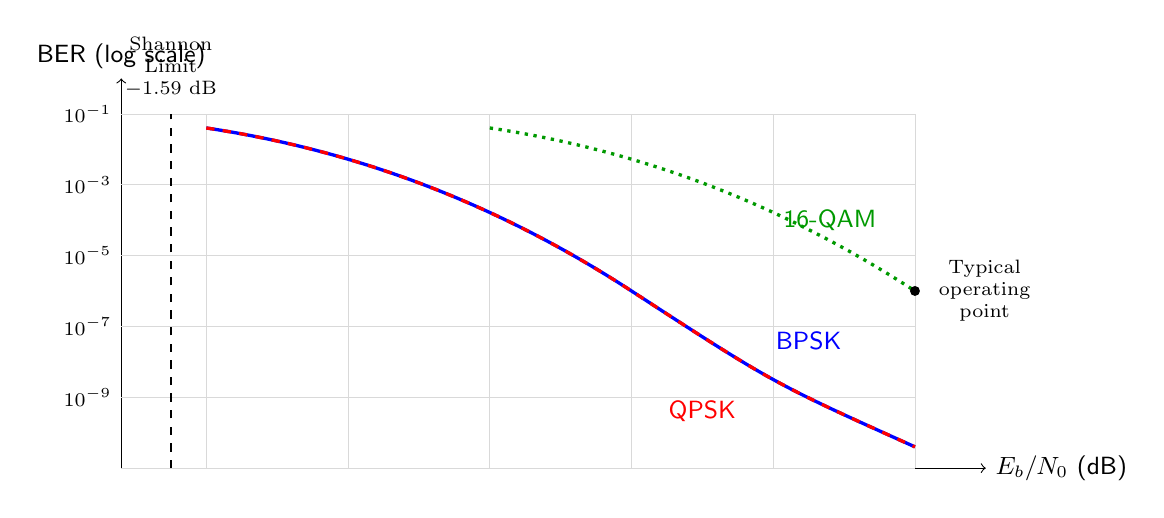
\begin{tikzpicture}[scale=0.90]
% Axes
\draw[->] (-1.2,0) -- (-1.2,5.5) node[above,font=\sffamily\small] {BER (log scale)};
\draw[->] (-1.2,0) -- (11,0) node[right,font=\sffamily\small] {$E_b/N_0$ (dB)};

% Grid
\foreach \x in {0,2,...,10} {
  \draw[very thin,gray!30] (\x,0) -- (\x,5);
}
\foreach \y in {0,1,...,5} {
  \draw[very thin,gray!30] (-1.2,\y) -- (10,\y);
}

% Y-axis labels (log scale BER)
\node[left,font=\scriptsize] at (-1.2,5) {$10^{-1}$};
\node[left,font=\scriptsize] at (-1.2,4) {$10^{-3}$};
\node[left,font=\scriptsize] at (-1.2,3) {$10^{-5}$};
\node[left,font=\scriptsize] at (-1.2,2) {$10^{-7}$};
\node[left,font=\scriptsize] at (-1.2,1) {$10^{-9}$};

% BPSK curve (approximately)
\draw[very thick,blue] (0,4.8) .. controls (2,4.5) and (4,3.8) .. (6,2.5) .. controls (8,1.2) .. (10,0.3);
\node[blue,font=\sffamily\small] at (8.5,1.8) {BPSK};

% QPSK curve (same as BPSK)
\draw[very thick,red,dashed] (0,4.8) .. controls (2,4.5) and (4,3.8) .. (6,2.5) .. controls (8,1.2) .. (10,0.3);
\node[red,font=\sffamily\small] at (7,0.8) {QPSK};

% 16-QAM curve (shifted right ~4 dB)
\draw[very thick,green!60!black,dotted] (4,4.8) .. controls (6,4.5) and (8,3.8) .. (10,2.5);
\node[green!60!black,font=\sffamily\small] at (8.8,3.5) {16-QAM};

% Shannon limit line
\draw[thick,dashed,black] (-0.5,0) -- (-0.5,5);
\node[font=\scriptsize,align=center,anchor=south] at (-0.5,5.1) {Shannon\\Limit\\$-1.59$~dB};

% Operating points
\fill[black] (10,2.5) circle (2pt);
\node[font=\scriptsize,align=center,anchor=west] at (10.2,2.5) {Typical\\operating\\point};

\end{tikzpicture}
\end{center}

\subsection{Relationship to SNR}

For systems with matched bandwidth, the relationship between $E_b/N_0$ and SNR is:
\begin{equation}
\frac{E_b}{N_0} = \mathrm{SNR} \cdot \frac{B}{R_b}
\end{equation}

In decibels:
\begin{equation}
\frac{E_b}{N_0}\bigg|_{\text{dB}} = \mathrm{SNR}_{\text{dB}} + 10\log_{10}\left(\frac{B}{R_b}\right)
\end{equation}

For Nyquist signaling ($B = R_b/2$):
\begin{equation}
\frac{E_b}{N_0}\bigg|_{\text{dB}} = \mathrm{SNR}_{\text{dB}} - 3.01~\text{dB}
\end{equation}

\section{Worked Example: Satellite Link}

\begin{calloutbox}{Problem Statement}
Design a QPSK satellite downlink to achieve BER $< 10^{-6}$. Calculate the required $E_b/N_0$ and verify link closure.

\textbf{System Parameters:}
\begin{itemize}
\item Modulation: QPSK (2 bits/symbol)
\item Data rate: $R_b = 2$~Mbps
\item Transmit power: $P_t = 10$~W (40~dBm)
\item TX antenna gain: $G_t = 35$~dBi
\item RX antenna gain: $G_r = 40$~dBi  
\item Distance: 36,000~km (GEO orbit)
\item Frequency: 12~GHz (Ku-band)
\item System noise temperature: $T_s = 150$~K
\item Implementation losses: 2~dB
\end{itemize}
\end{calloutbox}

\subsection*{Step 1: Required $E_b/N_0$}

For QPSK with BER $< 10^{-6}$, from the BER equation:
\begin{equation}
\mathrm{BER} = Q\left(\sqrt{\frac{2E_b}{N_0}}\right) = 10^{-6}
\end{equation}

Solving numerically: $E_b/N_0 = 10.5$~dB (theoretical)

Adding implementation losses and margin:
\begin{equation}
\left(\frac{E_b}{N_0}\right)_{\text{required}} = 10.5 + 2 + 3 = 15.5~\text{dB}
\end{equation}

\subsection*{Step 2: Free-Space Path Loss}

\begin{equation}
\mathrm{FSPL} = 20\log_{10}(d) + 20\log_{10}(f) + 32.45
\end{equation}
\begin{equation}
\mathrm{FSPL} = 20\log_{10}(36{,}000) + 20\log_{10}(12{,}000) + 32.45 = 205.5~\text{dB}
\end{equation}

\subsection*{Step 3: Received Signal Power}

\begin{equation}
P_r = P_t + G_t + G_r - \mathrm{FSPL}
\end{equation}
\begin{equation}
P_r = 40 + 35 + 40 - 205.5 = -90.5~\text{dBm}
\end{equation}

Converting to watts:
\begin{equation}
P_r = 10^{-90.5/10} \times 10^{-3} = 8.91 \times 10^{-13}~\text{W}
\end{equation}

\subsection*{Step 4: Noise Power Spectral Density}

\begin{equation}
N_0 = k_B T_s = (1.38 \times 10^{-23})(150) = 2.07 \times 10^{-21}~\text{W/Hz}
\end{equation}

In dBm/Hz:
\begin{equation}
N_0 = 10\log_{10}(2.07 \times 10^{-21} / 10^{-3}) = -176.8~\text{dBm/Hz}
\end{equation}

\subsection*{Step 5: Calculate Achieved $E_b/N_0$}

\begin{equation}
\frac{E_b}{N_0} = \frac{P_r}{N_0 \cdot R_b} = \frac{8.91 \times 10^{-13}}{(2.07 \times 10^{-21})(2 \times 10^6)} = 215.2
\end{equation}

In decibels:
\begin{equation}
\frac{E_b}{N_0}\bigg|_{\text{dB}} = 10\log_{10}(215.2) = 23.3~\text{dB}
\end{equation}

Or directly from power levels:
\begin{equation}
\frac{E_b}{N_0}\bigg|_{\text{dB}} = P_r - N_0 - 10\log_{10}(R_b)
\end{equation}
\begin{equation}
\frac{E_b}{N_0}\bigg|_{\text{dB}} = -90.5 - (-176.8) - 10\log_{10}(2 \times 10^6) = 23.3~\text{dB}
\end{equation}

\subsection*{Step 6: Link Margin}

\begin{equation}
\text{Margin} = E_b/N_0\big|_{\text{achieved}} - E_b/N_0\big|_{\text{required}} = 23.3 - 15.5 = 7.8~\text{dB}
\end{equation}

\begin{keyconcept}
The 7.8~dB link margin provides resilience against:
\begin{itemize}
\item Rain fade (5--8~dB at Ku-band)
\item Antenna pointing errors (1--2~dB)
\item Component aging and degradation
\item Atmospheric effects
\end{itemize}
\textbf{Conclusion:} Link is viable with adequate margin for reliable 2~Mbps QPSK operation.
\end{keyconcept}

\section{Applications}

\subsection{Link Budget Analysis}

Every communication system design begins with a link budget that calculates the required $E_b/N_0$:

\textbf{Design flow:}
\begin{enumerate}
\item Determine required BER from application requirements
\item Select modulation scheme and coding
\item Calculate required $E_b/N_0$ from BER curves
\item Add implementation losses and fade margins
\item Calculate available $E_b/N_0$ from link parameters
\item Verify positive link margin
\end{enumerate}

\subsection{Adaptive Modulation and Coding (AMC)}

Modern systems (LTE, 5G, WiFi) dynamically adjust modulation based on measured $E_b/N_0$:

\begin{center}
\begin{tabular}{@{}llr@{}}
\toprule
$E_b/N_0$ Range & Modulation & Data Rate \\
\midrule
$< 5$~dB & No link & 0~Mbps \\
5--10~dB & BPSK/QPSK & 10~Mbps \\
10--15~dB & 16-QAM & 40~Mbps \\
15--20~dB & 64-QAM & 80~Mbps \\
$> 20$~dB & 256-QAM & 120~Mbps \\
\bottomrule
\end{tabular}
\end{center}

\subsection{Deep-Space Communications}

Voyager spacecraft (24+ billion km from Earth) operate at extreme low $E_b/N_0$:

\begin{itemize}
\item Received power: $-196$~dBm
\item Data rate: 160~bps (BPSK)
\item Required $E_b/N_0$: $\sim$5~dB (with powerful FEC)
\item Achieved $E_b/N_0$: $\sim$7~dB (minimal margin)
\end{itemize}

Every fraction of a dB matters at interplanetary distances!

\subsection{Commercial Satellite Systems}

\textbf{Direct-to-home TV (Ku-band):}
\begin{itemize}
\item Modulation: QPSK or 8PSK
\item Target BER: $10^{-9}$ (quasi-error-free)
\item Typical $E_b/N_0$: 12--15~dB
\item Margin: 3--5~dB for rain fade
\end{itemize}

\textbf{Mobile satellite (L-band):}
\begin{itemize}
\item Modulation: QPSK (robust)
\item Target BER: $10^{-6}$ (voice quality)
\item Typical $E_b/N_0$: 8--10~dB
\item Challenge: Handheld terminals with small antennas
\end{itemize}

\subsection{Comparison: SNR vs $E_s/N_0$ vs $E_b/N_0$}

These metrics measure different aspects of signal quality:

\begin{center}
\begin{tabular}{@{}llp{5cm}@{}}
\toprule
Metric & Definition & Primary Use \\
\midrule
SNR & $\frac{P_s}{P_n}$ & General signal quality, analog systems \\[8pt]
$E_s/N_0$ & $\frac{P_s \cdot T_s}{N_0}$ & Symbol-level performance analysis \\[8pt]
$E_b/N_0$ & $\frac{P_s \cdot T_b}{N_0}$ & \textbf{Universal} metric for comparing digital systems \\
\bottomrule
\end{tabular}
\end{center}

\begin{calloutbox}{When to Use Which Metric}
\begin{itemize}
\item \textbf{Use $E_b/N_0$} for: System comparisons, theoretical analysis, specifications
\item \textbf{Use $E_s/N_0$} for: Demodulator design, symbol-level processing
\item \textbf{Use SNR} for: Analog systems, quick power measurements
\end{itemize}

\textbf{Key relationship:} For matched-filter receivers with symbol rate $R_s$ and bandwidth $B \approx R_s$:
\[
E_s/N_0 \approx \mathrm{SNR}
\]
\end{calloutbox}

\section{Summary}

\begin{center}
\begin{tabular}{@{}ll@{}}
\toprule
\textbf{Concept} & \textbf{Description} \\
\midrule
$E_b$ & Energy per information bit (joules) \\
$E_s$ & Energy per transmitted symbol (joules) \\
$N_0$ & Noise power spectral density (W/Hz) \\
$E_b/N_0$ & Universal performance metric (dimensionless) \\
$E_s/N_0$ & Symbol-level performance metric \\
Relationship & $E_s = k \cdot E_b$ where $k$ = bits/symbol \\
Shannon Limit & $E_b/N_0 > -1.59$~dB for reliable communication \\
Typical QPSK & Requires $E_b/N_0 \approx 10.5$~dB for BER $= 10^{-6}$ \\
\bottomrule
\end{tabular}
\end{center}

\vspace{10pt}

\textbf{Key conversions (dB):}

\begin{center}
\begin{tabular}{@{}llr@{}}
\toprule
Modulation & Bits/Symbol & $E_b/N_0$ to $E_s/N_0$ \\
\midrule
BPSK & 1 & $E_s/N_0 = E_b/N_0 + 0.00$~dB \\
QPSK & 2 & $E_s/N_0 = E_b/N_0 + 3.01$~dB \\
8PSK & 3 & $E_s/N_0 = E_b/N_0 + 4.77$~dB \\
16-QAM & 4 & $E_s/N_0 = E_b/N_0 + 6.02$~dB \\
64-QAM & 6 & $E_s/N_0 = E_b/N_0 + 7.78$~dB \\
256-QAM & 8 & $E_s/N_0 = E_b/N_0 + 9.03$~dB \\
\bottomrule
\end{tabular}
\end{center}

\begin{keyconcept}
\textbf{Why $E_b/N_0$ is Fundamental:}

\begin{enumerate}
\item \textbf{Rate-independent:} Normalizes by bit rate, enabling fair comparison
\item \textbf{Bandwidth-independent:} Not affected by pulse shaping or filtering
\item \textbf{Universal:} All theoretical limits and practical systems reference $E_b/N_0$
\item \textbf{Additive:} Can directly account for coding gain, implementation loss
\end{enumerate}

$E_b/N_0$ is the \textit{lingua franca} of digital communications---every engineer must master this concept.
\end{keyconcept}

\section{Further Reading}

\textbf{Related chapters in this book:}
\begin{itemize}
\item Chapter~\ref{ch:snr}: Signal-to-Noise Ratio (SNR) --- Power-based quality metrics
\item Chapter~\ref{ch:ber}: Bit Error Rate (BER) --- Performance characterization
\item Chapter~\ref{ch:awgn}: Additive White Gaussian Noise (AWGN) --- Channel model
\item Chapter~\ref{ch:bpsk}: Binary Phase-Shift Keying (BPSK) --- Optimal binary modulation
\item Chapter~\ref{ch:qpsk}: QPSK Modulation --- 2 bits per symbol
\item Chapter~\ref{ch:qam}: Quadrature Amplitude Modulation (QAM) --- Higher-order schemes
\item Chapter~\ref{ch:link-budget}: Complete Link Budget Analysis --- System design
\item Chapter~\ref{ch:shannon}: Shannon's Channel Capacity Theorem --- Fundamental limits
\item Chapter~\ref{ch:fec}: Forward Error Correction (FEC) --- Coding gain
\end{itemize}

\textbf{Standard references:}
\begin{itemize}
\item Proakis \& Salehi, \textit{Digital Communications} (5th ed.), Chapter 4
\item Sklar, \textit{Digital Communications} (2nd ed.), Chapter 4
\item Haykin \& Moher, \textit{Communication Systems} (5th ed.), Chapter 7
\end{itemize}

\textbf{Practical applications:}
\begin{itemize}
\item 3GPP specifications (LTE/5G performance requirements)
\item DVB-S2 (satellite broadcasting standards)
\item IEEE 802.11 (WiFi adaptive modulation)
\item Deep Space Network (JPL) documentation
\end{itemize}
